\chapter{Implementation}
\label{sec:implementation}
% Hier greift man einige wenige, interessante Gesichtspunkte der
% Implementierung heraus. Das Kapitel darf nicht mit Dokumentation oder
% gar Programmkommentaren verwechselt werden. Es kann vorkommen, daß
% sehr viele Gesichtspunkte aufgegriffen werden müssen, ist aber nicht
% sehr häufig. Zweck dieses Kapitels ist einerseits, glaubhaft zu
% machen, daß man es bei der Arbeit nicht mit einem "Papiertiger"
% sondern einem real existierenden System zu tun hat. Es ist sicherlich
% auch ein sehr wichtiger Text für jemanden, der die Arbeit später
% fortsetzt. Der dritte Gesichtspunkt dabei ist, einem Leser einen etwas
% tieferen Einblick in die Technik zu geben, mit der man sich hier
% beschäftigt. Schöne Bespiele sind "War Stories", also Dinge mit denen
% man besonders zu kämpfen hatte, oder eine konkrete, beispielhafte
% Verfeinerung einer der in Kapitel 3 vorgestellten Ideen. Auch hier
% gilt, mehr als 20 Seiten liest keiner, aber das ist hierbei nicht so
% schlimm, weil man die Lektüre ja einfach abbrechen kann, ohne den
% Faden zu verlieren. Vollständige Quellprogramme haben in einer Arbeit
% nichts zu suchen, auch nicht im Anhang, sondern gehören auf Rechner,
% auf denen man sie sich ansehen kann.




% Also kurzer Überblick über die Struktur schreiben, dann auf GRPC eingehen. Wenn GRPC erklärt wurde, würde ich den DC_rounds Service vorstellen. Dann pseudoartig auf die Funktionen eingehen und ein Diagram zeichnen.
%Wo gab es probleme bei der implementation? Es gab probleme bei der synchronisation der unterschiedlichen teilnehmer.-> unterschiedliche Sekunden. Außerdem war es neu, dass mehrere nutzer auf den selben servercode "zugreifen" und das parallele programmieren. die fork nicht vergessen.
% wo gibt es unterschiede? design von grpc eingehen, man kann keine Nachrichten weiterleiten mit grpc. Nur 2 verbindungen zwischen CLients möglich.vllt noch mehr?
The conceptual approach of the DC network was presented in Chapter 3. Nevertheless, smart grids are a real-world system and it must be shown that the theoretical solution can be implemented in a practical environment. This chapter deals with the implementation of the introduced protocol. It is described which technical tools were used and at which implementation steps problems occurred.
\section{Aufbau der praktischen Umsetzung}
A DC network was implemented with the same requirements as defined in chapter 3. For technical reasons, however, the exact same structure could not be implemented. If there are any deviations from the defined protocol, then these will be described and explained in this chapter.
4 Raspberrypis are used to realise the design, where 3 Raspberrypis simulate the SMGW and 1 Raspberrypi represents the electricity provider.  In the following, the Raspberrpis that represent the SMGW are called clients and the Raspberrypi that represents the power provider is simply referred to as the power provider. All clients have a communication link via Lan to the power provider. However, the clients do not have a physical connection to each other. As suggested in the protocol, the only way for the clients to communicate is through the power provider. After the clients join the DC network, the clients build their local sum and send it periodically to the power provider. The electricity provider adds up the local totals and stores the global total in an external text file. In a smart grid, electricity consumption is sent to the electricity provider every 15-60 minutes. Since the implementation is a demo, the sending interval is 10 seconds. In addition, the demo was implemented in such a way that after 4 messages a client fails and a corrective action must be taken. After that the client can re-enter the DC network. To avoid having to implement the application and the related network protocol, gRPC was used as a framework.\\
\\
\textbf{gRPC Remote Procedure Calls - GRPC}
%hier ein kleiner text
\\
\\
GRPC is an open source remote procedure call (RPC) system developed by Google since 2015. GRPC relies on a client-server structure and simplifies the construction of linked systems. With GRPC, so-called services can be defined. Each service allows to declare different functions that can communicate via a self-selected message format referred to as Protocol Buffers. Therefore on the client the functions are implemented, while the server runs the interface and processes the client requests. On the client there is a stub that holds the same functions that are on the server. In gRPC server and client can communicate with each other, although they were implemented in different programming languages. In this work, both server and client were implemented in Python. A simple application example is shown in Figure 4.1.
\begin{figure}[tbp]
  \centering
  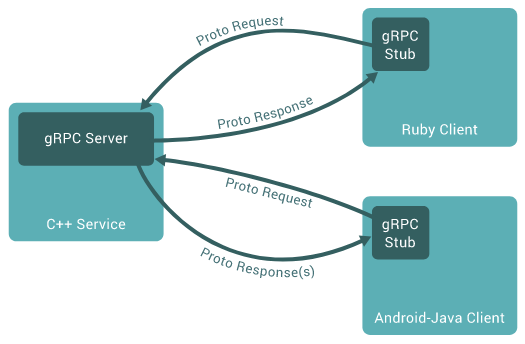
\includegraphics[width=0.8\textwidth]{images/grpc.png}
  \caption[Short description]{An example of a NILM analysis.}
  \label{fig:Appliance_Model}
\end{figure}\\
\\
\textbf{Protocol Buffers in gRPC}
%hier ein kleiner text
\\
\\
Protocol buffers are used by default in gRPC and allow structured data to be serialized. With Protocol Buffers, structured data can be specified as message formats. Then the source code is automatically generated from the structured data and it can be sent through channels provided by e.g. gRPC.
Listing 4.1 shows the implementation of the protocol header as a protocol buffer. Each header field is assigned a data type and also a unique field number that determines the order of the fields.\\
\lstinputlisting[language=protobuf2, style=protobuf,caption={%
Protocol Buffers message declaration using \texttt{protobuf/lang} and the
style in \texttt{protobuf/style}.}]{protobuf/dc_net.proto}\\
\\
\textbf{Client Implementation}
%hier ein kleiner text
\\
\\
When the application starts, a fork process is executed on client side. The fork process allows an application to create a second process by duplicating the address space of the calling process. The calling process is called parent and the duplicated process is called child. In the application, the parent process takes care of the child process. If the child process crashes, the parent process ensures that the child is restarted correctly. 
The actual logic of the application is located in the child process. First, the child establishes a connection to the electricity provider. The child receives a DC network identifier and a client ID. In the protocol from Chapter 3, it was described that the electricity provider must offer a tunnel so that two SMGWs can communicate with each other. But in gRPC all RPC requests are started by the client. The server only responds to the client's requests. Forwarding messages to non-requesting clients is therefore not possible or very difficult to implement in gRPC. Instead of the public keys being forwarded to the clients by the server, as suggested in the protocol, the public keys are stored on the server for a short time and the clients make a request for the public keys. After the Diffie Hellman key exchange has been executed and the PRNG has been configured, the client can create the local sum and send its local sum to the power provider/server for each round. The server calculates the global sum and verifies the correctness of the global sum. If the global sum is incorrect, then a client has failed and could not send a local sum. The client is located by the server and the neighboring clients are instructed by the server to resend the local sum without the key of the failed client. The global sum is then updated by the power provider. After each sending of the local sum, all clients check whether a new subscriber wants to register in the DC network. If so, the client is notified that it has a new neighbor. %den rest noch schreiben wie der CLient wieder verbunden wird und das jeder CLient nur 2 Verbindungen untereinander hat.
\\
\\
\textbf{Server Implementation}
\\
\\



%Den Service noch beschreiben!

%%% Local Variables:
%%% TeX-master: "diplom"
%%% End:

\cleardoublepage